\documentclass[ignorenonframetext,]{beamer}
\setbeamertemplate{caption}[numbered]
\setbeamertemplate{caption label separator}{: }
\setbeamercolor{caption name}{fg=normal text.fg}
\usepackage{lmodern}
\usepackage{amssymb,amsmath}
\usepackage{ifxetex,ifluatex}
\usepackage{fixltx2e} % provides \textsubscript
\ifnum 0\ifxetex 1\fi\ifluatex 1\fi=0 % if pdftex
  \usepackage[T1]{fontenc}
  \usepackage[utf8]{inputenc}
\else % if luatex or xelatex
  \ifxetex
    \usepackage{mathspec}
  \else
    \usepackage{fontspec}
  \fi
  \defaultfontfeatures{Ligatures=TeX,Scale=MatchLowercase}
  \newcommand{\euro}{€}
\fi
% use upquote if available, for straight quotes in verbatim environments
\IfFileExists{upquote.sty}{\usepackage{upquote}}{}
% use microtype if available
\IfFileExists{microtype.sty}{%
\usepackage{microtype}
\UseMicrotypeSet[protrusion]{basicmath} % disable protrusion for tt fonts
}{}
\newif\ifbibliography
\usepackage{color}
\usepackage{fancyvrb}
\newcommand{\VerbBar}{|}
\newcommand{\VERB}{\Verb[commandchars=\\\{\}]}
\DefineVerbatimEnvironment{Highlighting}{Verbatim}{commandchars=\\\{\}}
% Add ',fontsize=\small' for more characters per line
\usepackage{framed}
\definecolor{shadecolor}{RGB}{248,248,248}
\newenvironment{Shaded}{\begin{snugshade}}{\end{snugshade}}
\newcommand{\KeywordTok}[1]{\textcolor[rgb]{0.13,0.29,0.53}{\textbf{{#1}}}}
\newcommand{\DataTypeTok}[1]{\textcolor[rgb]{0.13,0.29,0.53}{{#1}}}
\newcommand{\DecValTok}[1]{\textcolor[rgb]{0.00,0.00,0.81}{{#1}}}
\newcommand{\BaseNTok}[1]{\textcolor[rgb]{0.00,0.00,0.81}{{#1}}}
\newcommand{\FloatTok}[1]{\textcolor[rgb]{0.00,0.00,0.81}{{#1}}}
\newcommand{\ConstantTok}[1]{\textcolor[rgb]{0.00,0.00,0.00}{{#1}}}
\newcommand{\CharTok}[1]{\textcolor[rgb]{0.31,0.60,0.02}{{#1}}}
\newcommand{\SpecialCharTok}[1]{\textcolor[rgb]{0.00,0.00,0.00}{{#1}}}
\newcommand{\StringTok}[1]{\textcolor[rgb]{0.31,0.60,0.02}{{#1}}}
\newcommand{\VerbatimStringTok}[1]{\textcolor[rgb]{0.31,0.60,0.02}{{#1}}}
\newcommand{\SpecialStringTok}[1]{\textcolor[rgb]{0.31,0.60,0.02}{{#1}}}
\newcommand{\ImportTok}[1]{{#1}}
\newcommand{\CommentTok}[1]{\textcolor[rgb]{0.56,0.35,0.01}{\textit{{#1}}}}
\newcommand{\DocumentationTok}[1]{\textcolor[rgb]{0.56,0.35,0.01}{\textbf{\textit{{#1}}}}}
\newcommand{\AnnotationTok}[1]{\textcolor[rgb]{0.56,0.35,0.01}{\textbf{\textit{{#1}}}}}
\newcommand{\CommentVarTok}[1]{\textcolor[rgb]{0.56,0.35,0.01}{\textbf{\textit{{#1}}}}}
\newcommand{\OtherTok}[1]{\textcolor[rgb]{0.56,0.35,0.01}{{#1}}}
\newcommand{\FunctionTok}[1]{\textcolor[rgb]{0.00,0.00,0.00}{{#1}}}
\newcommand{\VariableTok}[1]{\textcolor[rgb]{0.00,0.00,0.00}{{#1}}}
\newcommand{\ControlFlowTok}[1]{\textcolor[rgb]{0.13,0.29,0.53}{\textbf{{#1}}}}
\newcommand{\OperatorTok}[1]{\textcolor[rgb]{0.81,0.36,0.00}{\textbf{{#1}}}}
\newcommand{\BuiltInTok}[1]{{#1}}
\newcommand{\ExtensionTok}[1]{{#1}}
\newcommand{\PreprocessorTok}[1]{\textcolor[rgb]{0.56,0.35,0.01}{\textit{{#1}}}}
\newcommand{\AttributeTok}[1]{\textcolor[rgb]{0.77,0.63,0.00}{{#1}}}
\newcommand{\RegionMarkerTok}[1]{{#1}}
\newcommand{\InformationTok}[1]{\textcolor[rgb]{0.56,0.35,0.01}{\textbf{\textit{{#1}}}}}
\newcommand{\WarningTok}[1]{\textcolor[rgb]{0.56,0.35,0.01}{\textbf{\textit{{#1}}}}}
\newcommand{\AlertTok}[1]{\textcolor[rgb]{0.94,0.16,0.16}{{#1}}}
\newcommand{\ErrorTok}[1]{\textcolor[rgb]{0.64,0.00,0.00}{\textbf{{#1}}}}
\newcommand{\NormalTok}[1]{{#1}}
\usepackage{graphicx,grffile}
\makeatletter
\def\maxwidth{\ifdim\Gin@nat@width>\linewidth\linewidth\else\Gin@nat@width\fi}
\def\maxheight{\ifdim\Gin@nat@height>\textheight0.8\textheight\else\Gin@nat@height\fi}
\makeatother
% Scale images if necessary, so that they will not overflow the page
% margins by default, and it is still possible to overwrite the defaults
% using explicit options in \includegraphics[width, height, ...]{}
\setkeys{Gin}{width=\maxwidth,height=\maxheight,keepaspectratio}

% Prevent slide breaks in the middle of a paragraph:
\widowpenalties 1 10000
\raggedbottom

% Comment these out if you don't want a slide with just the
% part/section/subsection/subsubsection title:
\AtBeginPart{
  \let\insertpartnumber\relax
  \let\partname\relax
  \frame{\partpage}
}
\AtBeginSection{
  \ifbibliography
  \else
    \let\insertsectionnumber\relax
    \let\sectionname\relax
    \frame{\sectionpage}
  \fi
}
\AtBeginSubsection{
  \let\insertsubsectionnumber\relax
  \let\subsectionname\relax
  \frame{\subsectionpage}
}

\setlength{\emergencystretch}{3em}  % prevent overfull lines
\providecommand{\tightlist}{%
  \setlength{\itemsep}{0pt}\setlength{\parskip}{0pt}}
\setcounter{secnumdepth}{0}

\title{Notification Strategies for Tax Recovery}
\author{Michael Chirico\footnote<.->{The research presented here was supported
  in part by the Institute of Education Sciences, U.S. Department of
  Education, through Grant \#R305B090015 to the University of
  Pennsylvania. The opinions expressed are those of the presenter and do
  not represent the views of the Institute or the U.S. Department of
  Education.}, Robert Inman, Charles Loeffler, John MacDonald, Holger
Sieg}
\date{March 1, 2016}

\begin{document}
\frame{\titlepage}

\begin{frame}{Motivation}

\begin{itemize}
\item
  Tax non-compliance is ubiquitous in both developed and undeveloped
  economies

  \begin{itemize}
  \tightlist
  \item
    OECD estimates: 14.2\% in developed economies, 37\% in undeveloped
  \end{itemize}
\item
  The City of Philadelphia is currently owed \$413,814,249 in
  outstanding Real Estate Taxes.

  \begin{itemize}
  \item
    About 15\% of all properties in the city were out of compliance in
    March 2015.
  \item
    Roughly 5\% of the City's annual operating budget.
  \end{itemize}
\end{itemize}

\end{frame}

\begin{frame}{Motivation}

\begin{itemize}
\item
  Much existing literature focuses on sleight-of-hand -- non- or
  under-reporting of assets/income in environments where enforcement is
  scant or verifiability is costly.
\item
  No such fallback for real estate taxes

  \begin{itemize}
  \item
    Costs of establishing an office of assessment are sunk
  \item
    Exact tax value of each property is determined by the city and
    reported to the taxpayer (reversal)
  \end{itemize}
\item
  Alternative explanations

  \begin{itemize}
  \item
    Discontent with provided public goods
  \item
    Low tax morale
  \item
    Missing social norms
  \item
    Perceived unfairness of taxation
  \end{itemize}
\end{itemize}

\end{frame}

\begin{frame}{Motivation}

\begin{itemize}
\item
  Costs of containing culture of non-payment can quickly spiral

  \begin{itemize}
  \item
    Fewer people pay \(\Rightarrow\) harder to exact widespread
    compliance from a fixed budget \(\Rightarrow\) spread of
    noncompliance as perceived likelihood of apprehension decreases
  \item
    Cost of enforcement through augmented seizures can soon exceed
    potential recoveries
  \item
    To sustain public goods outlay, tax rates must rise -- potentially
    inducing further noncompliance
  \item
    Alternative of reduced expenditures may also create rogues through
    diminished tax morale
  \end{itemize}
\item
  Low-cost interventions offer a potential lighthouse in this hurricane
  spiral

  \begin{itemize}
  \item
    Targeted messaging in mailers
  \item
    Notification frequency
  \item
    Shape, color, style manipulation
  \item
    Public shaming
  \end{itemize}
\end{itemize}

\end{frame}

\begin{frame}{Overview of Treatments}

\begin{itemize}
\item
  Simultaneous (randomized) evaluation and head-to-head comparison of a
  variety of letter-based recovery nudges

  \begin{itemize}
  \item
    Message targeting: 3 pairs of treatments with wording varied to
    target different compliance motives
  \item
    Style cues: Half of treatments were delivered in large-format
    (\(9\)'`x \(12\)'')envelopes, the rest in standard-sized
    (\(4 \frac18\)'`x \(9 \frac12\)'') envelopes.
  \item
    Frequency: Some owners with multiple properties only received
    treatments on a subset of their holdings.
  \end{itemize}
\item
  All told, 15 treatment groups (including Holdout \& Control groups) on
  27,264 properties with 21,468 owners.
\end{itemize}

\end{frame}

\begin{frame}{Overview of Results}

\begin{itemize}
\item
  Evidence of strong initial effect for deterrence-oriented treatments

  \begin{itemize}
  \item
    Roughly NA\% higher participation (any payment) rates for owners in
    the Lien threat treament after one month.
  \item
    Also evidence of long-run effect mediation -- by the end of 2015
    (six months post-treatment), the advantage had shrunk to roughly
    NA\%.
  \end{itemize}
\item
  No evidence whatsoever that letter size affects compliance rates
\item
  Support for hypothesis that more letters lead to more participation
\end{itemize}

\end{frame}

\begin{frame}{Experimental Framework}

\end{frame}

\begin{frame}[fragile]{Slide with R Code and Output}

\begin{Shaded}
\begin{Highlighting}[]
\KeywordTok{summary}\NormalTok{(cars)}
\end{Highlighting}
\end{Shaded}

\begin{verbatim}
##      speed           dist       
##  Min.   : 4.0   Min.   :  2.00  
##  1st Qu.:12.0   1st Qu.: 26.00  
##  Median :15.0   Median : 36.00  
##  Mean   :15.4   Mean   : 42.98  
##  3rd Qu.:19.0   3rd Qu.: 56.00  
##  Max.   :25.0   Max.   :120.00
\end{verbatim}

\end{frame}

\begin{frame}{Slide with Plot}

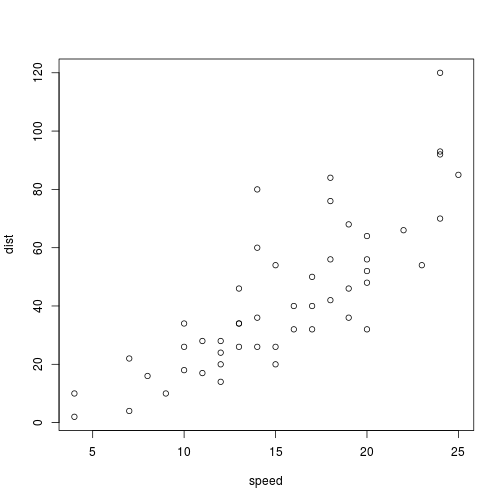
\includegraphics{micro_lunch_160301_files/figure-beamer/unnamed-chunk-2-1.pdf}

\end{frame}

\end{document}
